

\msection{Defensive Diversification: Speculative Side-channel protection}
\label{exploit:defensive}

As discussed in \autoref{sota:wasm}, \Wasm is quickly becoming a cornerstone technology in backend systems. 
Leading companies like Cloudflare and Fastly are championing the integration of \Wasm into their edge computing platforms, thereby enabling developers to deploy applications that are both modular and securely sandboxed. 
These server-side \Wasm applications are generally architected as isolated, single-responsibility services, a model referred to as Function-as-a-Service (FaaS) \cite{pMendkiServerless, 1244493Jacobsson}. 
The operational flow of \Wasm binaries in FaaS platforms is illustrated in \autoref{fig:edge_model}.

\begin{figure}[h]
    \centering
    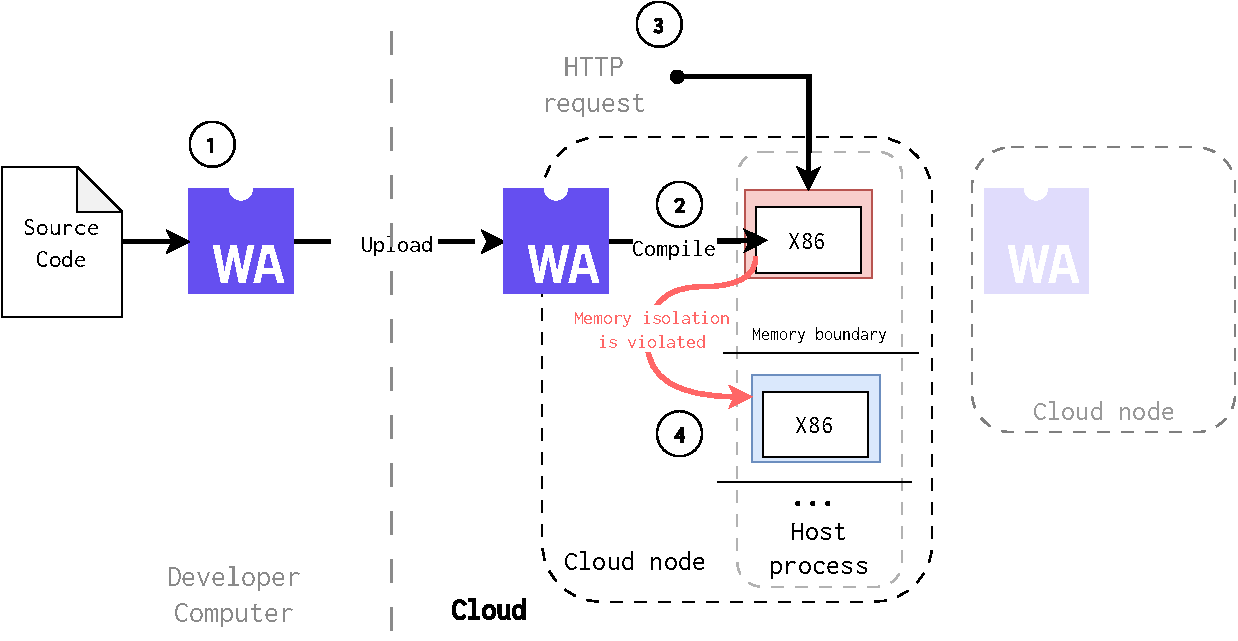
\includegraphics[width=0.8\linewidth]{figures/edge.pdf}
    \caption{\Wasm binaries on FaaS platforms. Developers can submit any \Wasm binary to the platform to be executed as a service in a sandboxed and isolated manner. Yet, \Wasm binaries are not immune to Spectre attacks.}
    \label{fig:edge_model}
\end{figure}


The fundamental advantage of using \Wasm in FaaS platforms lies in its ability to encapsulate thousands of client \Wasm binaries within a singular host process.
A developer could compile its source code into a \Wasm program suitable for the cloud platform and then submit it (\step{1} in \autoref{fig:edge_model}).
This host process is then disseminated across a network of servers and data centers (\step{2} in \autoref{fig:edge_model}). 
These platforms convert \Wasm programs into native code, which is subsequently executed in a sandboxed environment. 
Host processes can then instantiate new \Wasm sandboxes for each client function, executing them in response to specific user requests with nanosecond-level latency (\step{3} in \autoref{fig:edge_model}). 
This architecture inherently isolates \Wasm binary executions from each other as well as from the host process, enhancing security.

However, while \Wasm is engineered with a strong focus on security and isolation, it is not entirely immune to vulnerabilities such as Spectre attacks \cite{Spectre,Narayan2021Swivel} (\step{4} in \autoref{fig:edge_model}). 
In the sections that follow, we explore how software diversification techniques can be employed to harden \Wasm binaries against such attacks. For an in-depth discussion on this topic, we direct the reader to our contribution \cite{wasmmutate}.

\msubsection{Threat model: speculative side-channel attacks}

To illustrate the threat model concerning \Wasm programs in FaaS platforms, consider the following scenarios. 
Developers, including potentially malicious actors, have the ability to submit any \Wasm binary to the FaaS platform. 
A malicious actor could then upload a \Wasm binary that, once compiled to native code, employs Spectre attacks to either leak sensitive information from the host process or violate Control Flow Integrity (CFI).
Spectre attacks exploit hardware-based prediction mechanisms to trigger mispredictions, leading to the speculative execution of specific instruction sequences that are not part of the original, sequential execution flow. 
By taking advantage of this speculative execution, an attacker can potentially access sensitive information stored in the memory allocated to other \Wasm instance (including itself) or even the host process. 
Therefore, this poses a significant risk for the overall execution system.

Narayan and colleagues \cite{Narayan2021Swivel} have categorized potential Spectre attacks on \Wasm binaries into three distinct types, each corresponding to a specific hardware predictor being exploited and a particular FaaS scenario: Branch Target Buffer Attacks,  Return Stack Buffer Attacks, and Pattern History Table Attacks defined as follows:

\begin{enumerate}
    \item The Spectre Branch Target Buffer (btb) attack exploits the branch target buffer by predicting the target of an indirect jump, thereby rerouting speculative control flow to an arbitrary target.
    \item  The Spectre Return Stack Buffer (rsb) attack exploits the return stack buffer that stores the locations of recently executed call instructions to predict the target of \texttt{ret} instructions.
    \item The Spectre Pattern History Table (pht) takes advantage of the pattern history table to anticipate the direction of a conditional branch during the ongoing evaluation of a condition.
\end{enumerate}


%\lipsum[1]

%\lipsum[1]

\msubsection{Methodology}

Our goal is to empirically validate that Software Diversification can effectively mitigate the risks associated with Spectre attacks in \Wasm binaries. 
The green-highlighted section in \autoref{fig:defense_model} illustrates how Software Diversification can be integrated into the FaaS platform workflow. 
The core idea is to generate unique and diverse \Wasm variants that can be randomized at the time of deployment. 
For this use case, we employ WASM-MUTATE as our tool for Software Diversification.

To empirically demonstrate that Software Diversification can indeed mitigate Spectre vulnerabilities, we reuse the \Wasm attack scenarios proposed by Narayan and colleagues in their work on Swivel \cite{Swivel}. 
Swivel is a compiler-based strategy designed to counteract Spectre attacks on \Wasm binaries by linearizing their control flow during machine code compilation. 
Our approach differs from theirs in that it is binary-based, compiler-agnostic, and platform-agnostic; we do not propose altering the deployment or toolchain of FaaS platforms. 


\begin{figure}[h]
    \centering
    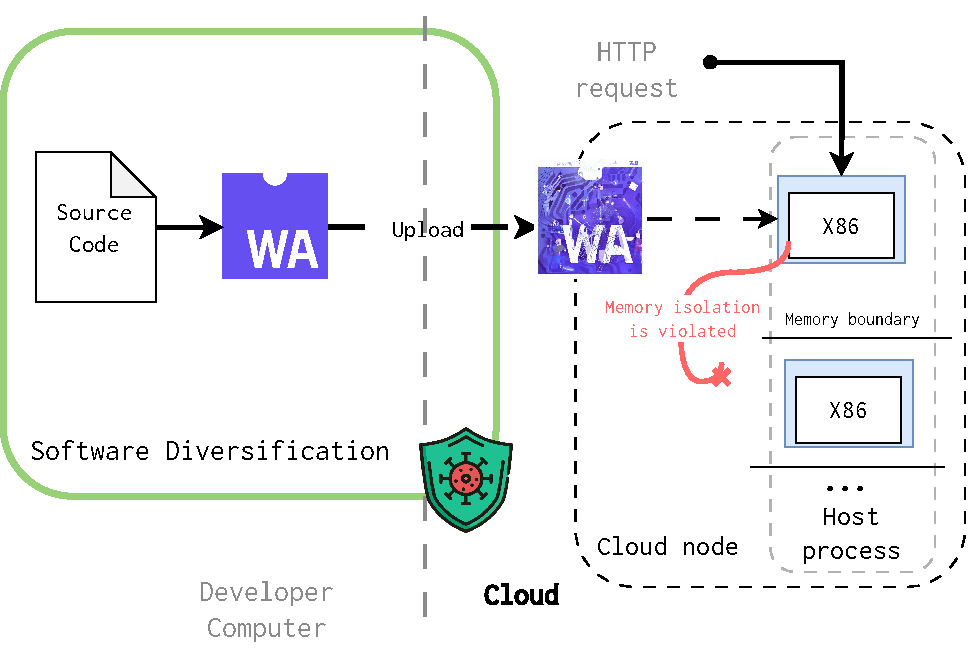
\includegraphics[width=0.75\linewidth]{figures/edge_protected.pdf}
    \caption{Diversifying \Wasm binaries to mitigate Spectre attacks in FaaS platforms.}
    \label{fig:defense_model}
\end{figure}

\begin{table}
    \centering
    \begin{tabular}{l | l  }
        \hline
         Program &  Attack  \\
        \hline \hline
        btb\_breakout & Spectre branch target buffer (btb)  \\
        \hline
         btb\_leakage & Spectre branch target buffer (btb)  \\
        \hline
         ret2spec &  Spectre Return Stack Buffer (rsb)  \\
        \hline
        pht &  Spectre Pattern History Table (pht)  \\

%\end{adjustbox}
    \end{tabular}
    \caption{\Wasm program name and its respective attack.}
    \label{programs}
\end{table}

To measure the efficacy of WASM-MUTATE in mitigating Spectre, we diversify four \Wasm binaries proposed in the Swivel study. 
The names of these programs and the specific attacks we examine are available in \autoref{programs}. 
For each of these four binaries, we generate up to 1000 random stacked transformations (see \autoref{stack_transform}) using 100 distinct seeds, resulting in a total of 100,000 variants for each original binary. 
At every 100th stacked transformation for each binary and seed, we assess the impact of diversification on the Spectre attacks by measuring the attack bandwidth for data exfiltration. 
This metric not only captures the success or failure of the attacks but also quantifies the extent to which data exfiltration is hindered. 
For example, a variant that still leaks data but does so at an impractically slow rate would be considered hardened against the attack.

\begin{definition}{Attack bandwidth:}\label{metric:ber}
    Given data $D=\{b_0, b1, ..., b_C\}$ being exfiltrated in time $T$ and $K = {k_1, k_2, ..., k_N}$ the collection of correct data bytes, the bandwidth metric is defined as:
    $$
        \frac{|b_i\text{ such that } b_i \in K|}{T}
    $$
\end{definition}


\msubsection{Results}


\autoref{attacks:impact:1} offers a graphical representation of \tool's influence on the Swivel original programs: btb\_breakout and btb\_leakage with the btb attack. 
The Y-axis represents the exfiltration bandwidth (see \autoref{metric:ber}). 
The bandwidth of the original binary under attack is marked as a blue dashed horizontal line.
In each plot, the variants are grouped in clusters of 100 stacked transformations. 
These are indicated by the green violinplots.

\begin{figure}[h]
    \centering
    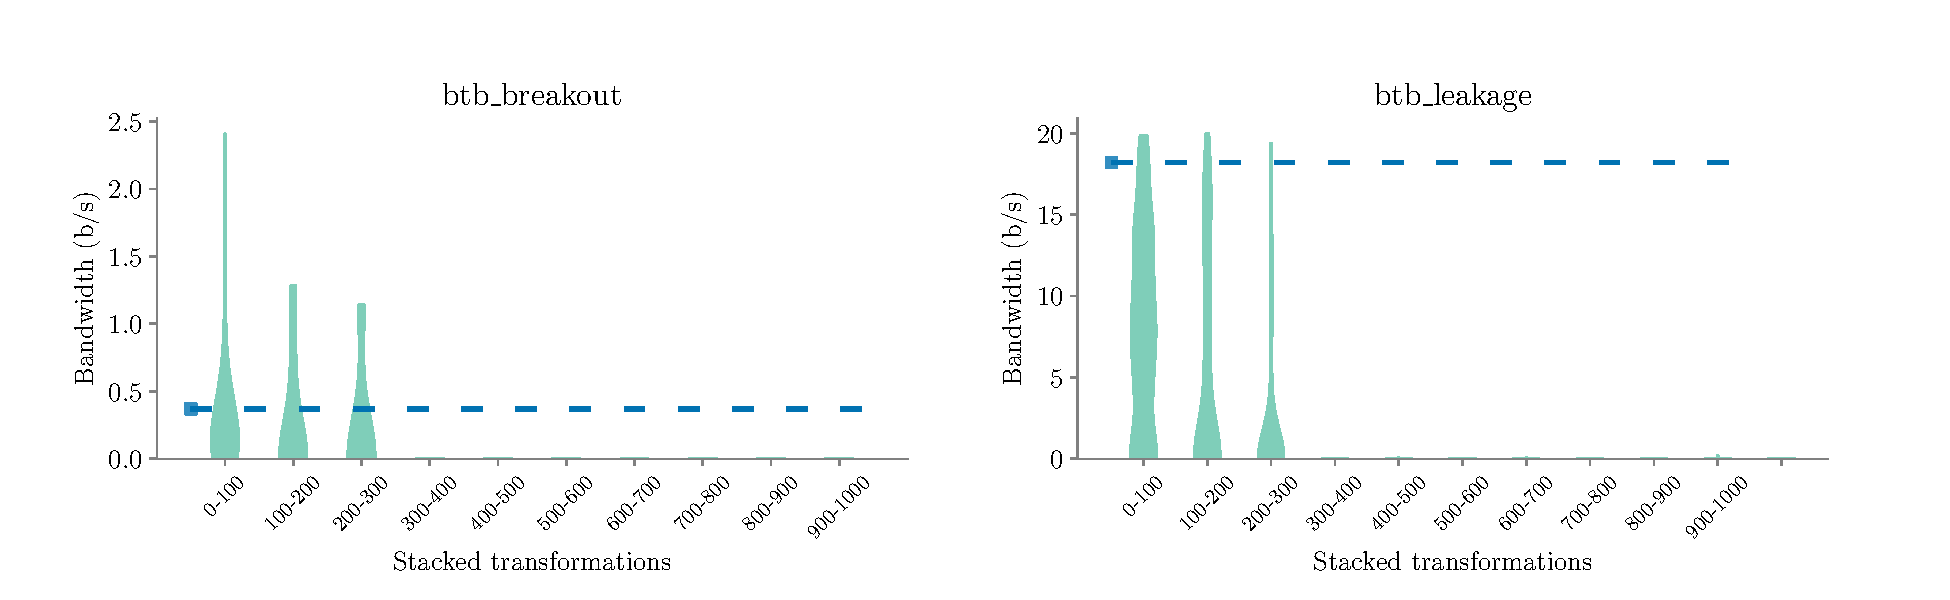
\includegraphics[width=\linewidth]{plots/spectre/results.rq3.1.pdf}
    \caption{Impact of WASM-MUTATE over btb\_breakout and btb\_leakage binaries. The Y-axis denotes exfiltration bandwidth, with the original binary's bandwidth under attack highlighted by a blue marker and dashed line. Variants are clustered in groups of 100 stacked transformations, denoted by green violinplots. 
    Overall, for all 100000 variants generated out of each original program, 70\% have less data leakage bandwidth.
    After 200 stacked transformations, the exfiltration bandwidth drops to zero.
    }
  \label{attacks:impact:1}
\end{figure}

\wrule{Population Strength:} For the binaries btb\_breakout and btb\_leakage, \tool exhibits a high level of effectiveness, generating variants that leak less information than the original in 78\% and 70\% of instances, respectively.
For both programs, after applying 200 stacked transformations, the exfiltration bandwidth drops to zero.
This implies that \tool is capable of synthesizing variants that are entirely protected from the original attack.
If we consider the results in \autoref{comp:table:tools}, generating a variant with 200 stacked transformations can be accomplished in just a matter of seconds for a single \Wasm binary.
When scaled to the scope of a global FaaS platform, this means that a unique, hardened variant could be deployed for each machine and even for each fresh \Wasm spawned per user request.

\begin{figure}[h]
    \centering    
    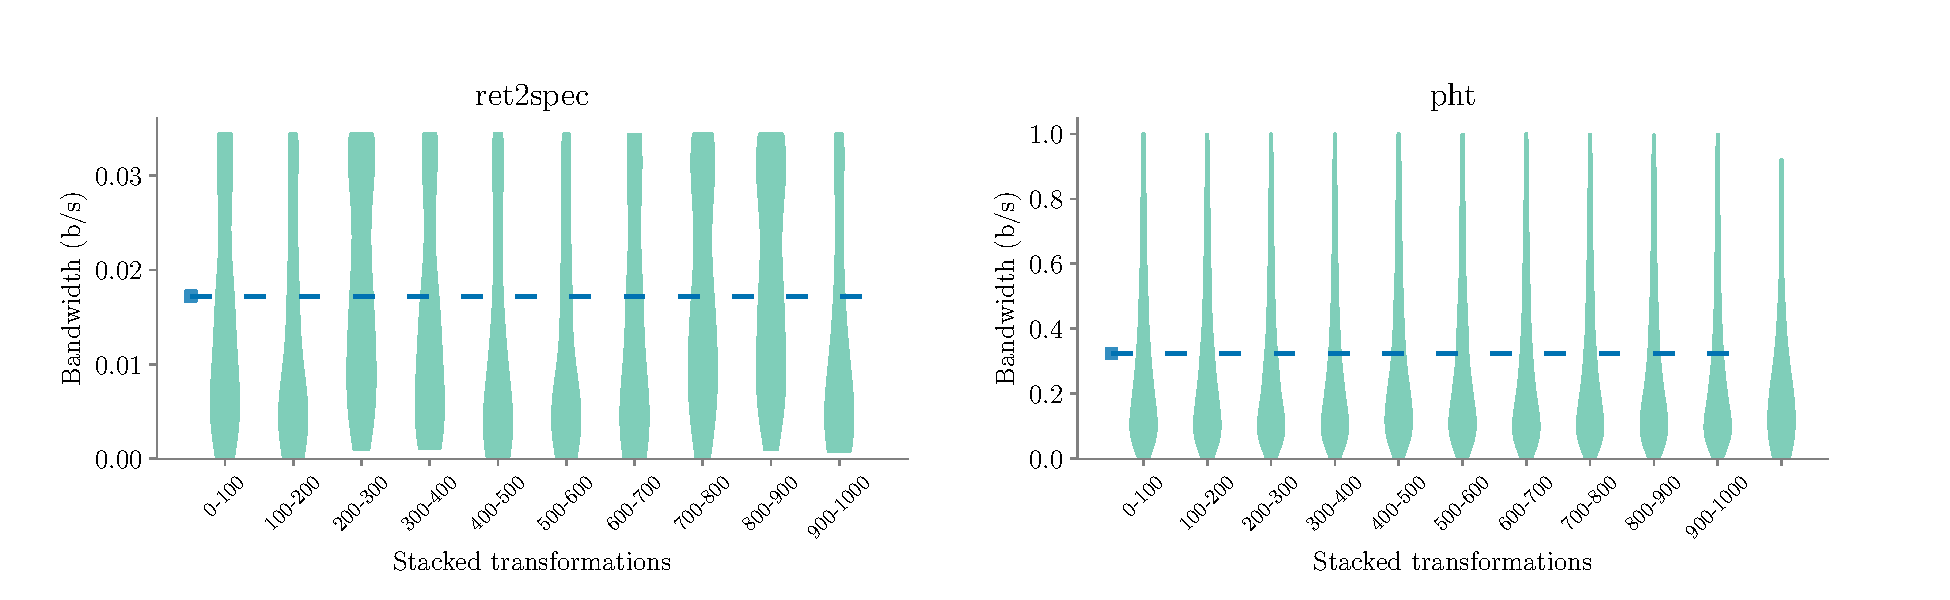
\includegraphics[width=\linewidth]{plots/spectre/results.rq3.2.pdf}
    \caption{Impact of WASM-MUTATE over ret2spec and pht binaries. The Y-axis denotes exfiltration bandwidth, with the original binary's bandwidth under attack highlighted by a blue marker and dashed line. Variants are clustered in groups of 100 stacked transformations, denoted by green violinplots. 
    Overall, for both programs approximately 70\% of the variants have less data leakage bandwidth.}
  \label{attacks:impact:2}
\end{figure}


% \todo{replace with violin plots}
As illustrated in \autoref{attacks:impact:2}, similarly to \autoref{attacks:impact:1}, WASM-MUTATE significantly impacts the programs ret2spec and pht when subjected to their respective attacks. 
In 76\% of instances for ret2spec and 71\% for pht, the generated variants demonstrated reduced attack bandwidth compared to the original binaries.
The plots reveal that a notable decrease in exfiltration bandwidth occurs after applying at least 100 stacked transformations. 
While both programs show signs of hardening through reduced attack bandwidth, this effect is not immediate and requires a substantial number of transformations to become effective. 
Additionally, the bandwidth distribution is more varied for these two programs compared to the two previous ones.
Our analysis suggests a correlation between the reduction in attack bandwidth and the complexity of the binary being diversified. 
Specifically, ret2spec and pht are substantially larger programs, containing over 300,000 instructions, compared to btb\_breakout and btb\_leakage, which have fewer than 800 instructions. 
Therefore, given that WASM-MUTATE performs one transformation per invocation, the probability of affecting critical components to hinder attacks decreases in larger binaries.

\wrule{Managed memory impact:} The success in diminishing Spectre attacks is explained by the fact that \tool synthesizes variants that effectively alter memory access patterns. 
We have identified four primary factors responsible for the divergence in memory accesses among \tool generated variants.
First, modifications to the binary layout—even those that do not affect executed code—inevitably alter memory accesses within the program's stack. 
Specifically, \tool generates variants that modify the return addresses of functions, which consequently leads to differences in execution flow and memory accesses.
Second, one of our rewriting rules incorporates artificial global values into \Wasm binaries. 
The access to these global variables inevitably affects the managed memory (see \autoref{background:wasm:execution}).
Third, \tool injects 'phantom' instructions which do not aim to modify the outcome of a transformed function during execution. 
These intermediate calculations trigger the spill/reload component of the wasmtime compiler, varying spill and reload operations. 
In the context of limited physical resources, these operations temporarily store values in memory for later retrieval and use, thus creating diverse managed memory accesses (see the example at \autoref{custom}).
Finally, certain rewriting rules implemented by WASM-MUTATE replicate fragments of code, e.g., performing commutative operations. 
These code segments may contain memory accesses, and while neither the memory addresses nor their values change, the frequency of these operations does.



% \subsection{Deoptimization}

\begin{tcolorbox}[title=Contribution paper,boxrule=1pt,arc=.2em,boxsep=1.0mm]
    WASM-MUTATE crafts \Wasm binaries that are resilient to Spectre-like attacks. 
    By integrating a software diversification layer into \Wasm binaries deployed on Function-as-a-Service (FaaS) platforms, security can be significantly bolstered. 
    This approach allows for the deployment of unique and diversified \Wasm binaries, potentially utilizing a distinct variant for each cloud node, thereby enhancing the overall security.
    The case discussed in this section is fully detailed in Cabrera-Arteaga \etal "WASM-MUTATE: Fast and Effective Binary Diversification for WebAssembly"
    \emph{Under review}
    \url{https://arxiv.org/pdf/2309.07638.pdf}. 
\end{tcolorbox}



